\documentclass[12pt]{extarticle}
%Some packages I commonly use.
\usepackage[english]{babel}
\usepackage{graphicx}
\usepackage{framed}
\usepackage[normalem]{ulem}
\usepackage{amsmath}
\usepackage{amsthm}
\usepackage{amssymb}
\usepackage{amsfonts}
\usepackage{enumerate}
\usepackage[utf8]{inputenc}
\usepackage[top=1 in,bottom=1in, left=1 in, right=1 in]{geometry}
% \usepackage{xeCJK}
\usepackage{physics}
\usepackage{hyperref}
\usepackage{multicol}

% \usepackage{tabularx,booktabs}


% \graphicspath{ {./images/} }
\numberwithin{equation}{section}
\numberwithin{figure}{section}
\numberwithin{table}{section}


%A bunch of definitions that make my life easier
\newcommand{\matlab}{{\sc Matlab} }
\newcommand{\cvec}[1]{{\mathbf #1}}
\newcommand{\rvec}[1]{\vec{\mathbf #1}}
\newcommand{\ihat}{\hat{\textbf{\i}}}
\newcommand{\jhat}{\hat{\textbf{\j}}}
\newcommand{\khat}{\hat{\textbf{k}}}
\newcommand{\minor}{{\rm minor}}
% \newcommand{\trace}{{\rm trace}}
\newcommand{\spn}{{\rm Span}}
\newcommand{\rem}{{\rm rem}}
\newcommand{\ran}{{\rm range}}
\newcommand{\range}{{\rm range}}
\newcommand{\mdiv}{{\rm div}}
\newcommand{\proj}{{\rm proj}}
\newcommand{\R}{\mathbb{R}}
\newcommand{\N}{\mathbb{N}}
\newcommand{\Q}{\mathbb{Q}}
\newcommand{\Z}{\mathbb{Z}}
\newcommand{\<}{\langle}
\renewcommand{\>}{\rangle}
\renewcommand{\emptyset}{\varnothing}
\newcommand{\attn}[1]{\textbf{#1}}
\theoremstyle{definition}
\newtheorem{theorem}{Theorem}
\newtheorem{corollary}{Corollary}
\newtheorem*{definition}{Definition}
\newtheorem*{example}{Example}
\newtheorem*{note}{Note}
\newtheorem{exercise}{Exercise}
\newcommand{\bproof}{\bigskip {\bf Proof. }}
\newcommand{\eproof}{\hfill\qedsymbol}
\newcommand{\Disp}{\displaystyle}
\newcommand{\qe}{\hfill\(\bigtriangledown\)}

\newcommand{\SubItem}[1]{
    {\setlength\itemindent{15pt} \item[-] #1}
}


\setlength{\columnseprule}{1 pt}


\title{Nonlinear Fiber Optics\cite{agrawal_nonlinear_2007} Summary}
\author{Maodong Gao}
\date{\today}

\begin{document}

\maketitle

\section{Introduction}

    \subsection{Historical prospective}
    
        \begin{itemize}
            \item 1960, fibres lossy $\geq$ 1000dB/km. 1970 20dB/km.
            \item 1979, loss level 0.2dB/km in 1.55um. Limited by Rayleigh Scattering.
            \item 1972, Raman and Brillouin scattering process are studied using optical fibers.
            \item Stimulated other nonlinear phenomena,including optically induced birefringence, parametric 4-wave mixing, self-phase modulation
            \item 1973, soliton like pulses are suggested. 1980 observed. 6fs pulse observed in 1987.
            \item 1990s, Erbium-doped fiber amplifier, wavelength near 1550nm.
            \item 2000s, stimulated Raman scattering(so called Raman amplification), four-wave mixing(so called Fiber-optic parametric amplifiers) are two new types of amplifiers. Do not require doped atoms and spectral region not limited.
            \item Amplifiers fueled optical solitons. New types of solitons such as dispersion-managed solitons and dissipative solitons.
            \item (Chapter 11) 1978, fibre gratings. 1996, New types of fibers, such as photonic crystal fibres, crystal fibers,  holey fibers and micro-structure fibers.
            \item (Chapter 12) New types of fibers has new dispersive (GVD, group velocity dispersion) and nonlinear (relativity small core size enhance nonlinear effects) properties.
            \item (Chapter 13) Supercontinuum generation. optical spectrum of incident light broadens by a factor of $\geq$100 over a short length of fiber.
        \end{itemize}
    
    \subsection{Fiber Characteristics}
        \begin{itemize}
            \item step-index fibers, see \autoref{fig1.1}.
            \item Two parameters characterize optical fiber: relative core-cladding index difference; V parameter.
            \item core-cladding index difference:
                \begin{equation}
                    \Delta = \frac{n_1 - n_c}{n_1}
                    \label{core-cladding index difference}
                \end{equation}
            \item V parameter: this parameter determines number of modes supported by this fiber at a certain wavelength $\lambda$. Fiber supports single mode of a certain $\lambda$ if $V < 2.405$.
                \begin{equation}
                    V = k_0 a \sqrt{n_1^2 - n_c^2}
                    \label{V parameter}
                \end{equation}
            where a is core radius, $k_0 = \frac{2\pi}{\lambda}$
        \end{itemize}
    
        \begin{figure}[htbp]
            \centering
            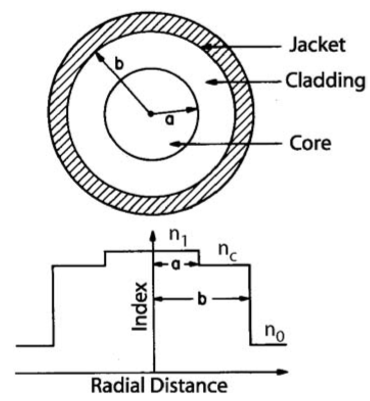
\includegraphics[width=0.4\textwidth]{images/fig1.1.PNG}
            \caption{Schematic illustration of the cross section and the refractive-index profile of a stepindex fiber.}
            \label{fig1.1}
        \end{figure}
        
        \subsubsection{Material and Fabrication}
            \begin{figure}[htbp]
                \centering
                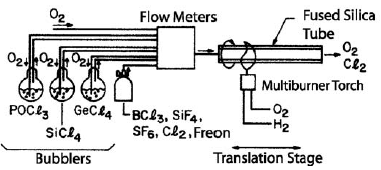
\includegraphics[width=0.6\textwidth]{images/fig1.2.PNG}
                \caption{Schematic diagram of the MCVD process commonly used for fiber fabrication.}
                \label{fig1.2}
            \end{figure}
            
            \begin{itemize}
                \item Dopants increase refractive index: $GeO_2, P_2O_5$.
                \item Dopants decrease refractive index: $boron, fluorine$
                \item Dopants to core for amplification: $ErCl_3, Nd_2O_3$
                \item MCVD(modified chemical vapor deposition) fiber fabrication process.
            \end{itemize}
            
        \subsubsection{Fiber Losses}
            Losses are characterized by attenuation constant $\alpha$:
                \begin{equation}
                    P_T = P_0 \exp{(-\alpha L)}.
                    \label{attenuation constant}
                \end{equation}
            Another unit for $\alpha$ is dB/km, which are related by:
                \begin{equation}
                    \alpha_{dB} = -\frac{10}{L}\log{(\frac{P_T}{P_0})} = 4.343\alpha
                \end{equation}
            A high loss up to 10dB/km corresponds to attenutation constant of \\
            $\alpha \approx 2 km^{-1} = 2\times 10^{-5}cm^{-1} $,
            which is already very low compared to most other materials.
            
            
            \begin{figure}[htbp]
                \centering
                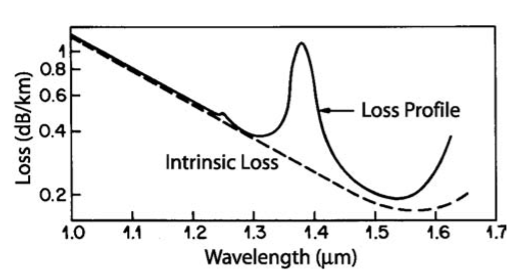
\includegraphics[width=0.6\textwidth]{images/fig1.3.PNG}
                \caption{Measured loss spectrum of a single-mode silica fiber. Dashed curve shows the contribution resulting from Rayleigh scattering.}
                \label{fig1.3}
            \end{figure}
            
            Two main fiber loss channels: Rayleigh scattering; Material absorption.
            \begin{itemize}
                \item Raleigh scattering, arises from density fluctuation frozen into fused silica.Local fluctuations in refractive index, scatter lights into all directions.
                    \begin{equation}
                        \alpha_R = \frac{C_R}{\lambda^4}
                    \end{equation}
                    Raleigh scattering strength decreases rapidly as wavelength increases. $C_R$ depends on constituents of fiber core, typically around $0.7-0.9 dB/(km \mu m^4)$. As $\alpha_R$ around $0.12-0.15 dB/km$ near $\lambda = 1.55 \mu m$.
                \item Material absorption: Silica glass electronic resonance (ultraviolet region), vibrational resonance (far-infrared region beyond $2 \mu m$). Absorbs little light from $0.5 \mu m$ to $2 \mu m$.
                \item Impurity absorption: most important impurity is OH ion. Its fundamental vibrational absorption peak is at $\approx 2.73 \mu m$. The peak in \autoref{fig1.3} is the second overtone of OH ions.
            \end{itemize}
            
        \subsubsection{Chromatic Dispersion}
            \begin{itemize}
                \item Chromatic dispersion basically is reflective index over optical frequency $n(\omega)$.
                \item $n(\omega)$ relation with material resonance is well approximated by Sellmeier equation:
                    \begin{equation}
                        n^2(\omega) = 1 + \sum_{j=1}^m \frac{B_j \omega_j^2}{\omega_j^2-\omega^2},
                        \label{sellmeier equation}
                    \end{equation}
                    where $\omega_j$ are material resonances frequencies, $B_j$ is the strength of $j$th resonance. $\omega_j$ contributes more as it is nearer to frequcney of interest $\omega$.
                \item For bulk-fused silica, the fitting of Sellmeier equation to $m = 3$ has the parameters in \autoref{bulk-fused silica Sellmeier equation fitting}. This is useful when doing COMSOL simulation. The $n(\omega)$ results are shown in \autoref{fig1.4}.
                    \begin{table}[htbp]
                    \centering
                        \begin{tabular}{|c|c|c|c|}
                        \hline
                        \multicolumn{4}{|c|}{Fitting coefficients in \autoref{sellmeier equation} for bulk-fused silica up to order m=3} \\
                        \hline
                        $j$ in \autoref{sellmeier equation} & 1       & 2           & 3           \\ \hline
                        $B_j$                          & 0.6961663   & 0.4079426   & 0.8974794   \\ \hline
                        $\lambda_j / nm$               & 68.4043     & 116.2414    & 9896.161    \\ \hline
                        $\omega_j =2\pi c/\lambda_j$   & 2.7537E+16  & 1.62047E+16 & 1.90342E+14 \\ \hline
                        Freq /THz                      & 43.82655155 & 25.79050648 & 0.302938137 \\ \hline
                        \end{tabular}
                    \caption{bulk-fused silica Sellmeier \autoref{sellmeier equation} fitting}
                    \label{bulk-fused silica Sellmeier equation fitting}
                    \end{table}
                \item Dispersion induce short optical pulse broadening.
                \item Dispersion and non-linearity are different behavior components. In nonlinear regime, these two may behave qualitatively different.
                
                \item Group index $n_g$: Define $n_g = \frac{v_g}{c}$. From mode-propagation constant $\beta$ view, Taylor expands $\beta(\omega)$ about the center pulse freq $\omega_0$, 
                    \begin{equation}
                        \beta(\omega) = n(\omega)\frac{\omega}{c}=\beta_0 + \beta_1(\omega-\omega_0)+\frac{1}{2}\beta_2(\omega-\omega_0)^2,
                        \label{propagation constant expansion}
                    \end{equation}
                    where
                    \begin{equation}
                        \beta_m = (\dv[m]{\beta}{\omega})_{\omega=\omega_0}.
                        \label{betam definition}
                    \end{equation}
                    And $n_g$ are related to $\beta_1$ by:
                    \begin{equation}
                        \beta_1 = \frac{1}{v_g} = \frac{n_g}{c} = \frac{1}{c}(n+\omega \dv{n}{\omega}).
                        \label{group velocity and group index}
                    \end{equation}
                
                \item Group velocity dispersion (GVD): characterized by $\dv{n_g}{\omega}$, and this is related to $\beta_2$ by:
                    \begin{equation}
                        \beta_2 = \dv{\beta_1}{\omega} = \frac{1}{c}\dv{n_g}{\omega} = \frac{1}{c}(2\dv{n}{\omega} +\dv[2]{n}{\omega}).
                        \label{beta2 definition}
                    \end{equation}
                    
                \item GVD parameter D: Defined by $\dv{\beta_1}{\lambda}$. Related to $\beta_2$ by:
                    \begin{equation}
                        D = \dv{\beta_1}{\lambda} = -\frac{2\pi c}{\lambda^2}\beta_2 = -\frac{\lambda}{c}\dv[2]{n}{\lambda}
                        \label{D2 definition}
                    \end{equation}
                     The results of \autoref{beta2 definition} and \autoref{D2 definition} are illustrated in \autoref{fig1.5}, based on the calculation of \autoref{sellmeier equation}.
                     
                \item Normal and Anomalous dispersion: divided by the sign of D.
                    \begin{table}[htbp]
                    \centering
                    \begin{tabular}{|c|c|c|c|}
                        \hline
                        Normal dispersion    & $\beta_2$\textgreater{}0 & $D_2$\textless{}0    & red fast  \\ \hline
                        Anomalous dispersion & $\beta_2$\textless{}0    & $D_2$\textgreater{}0 & blue fast \\ \hline
                    \end{tabular}
                    \caption{Summary of normal and anomalous dispersion.}
                    \label{Summary of normal and anomalous dispersion}
                    \end{table}
                    
                    Anomalous dispersion regime is the regime optical fibers support solitons. Solitons are self-formed by a process of balancing dispersive and nonlinear effects.
                    \begin{figure}[htbp]
                        \centering
                        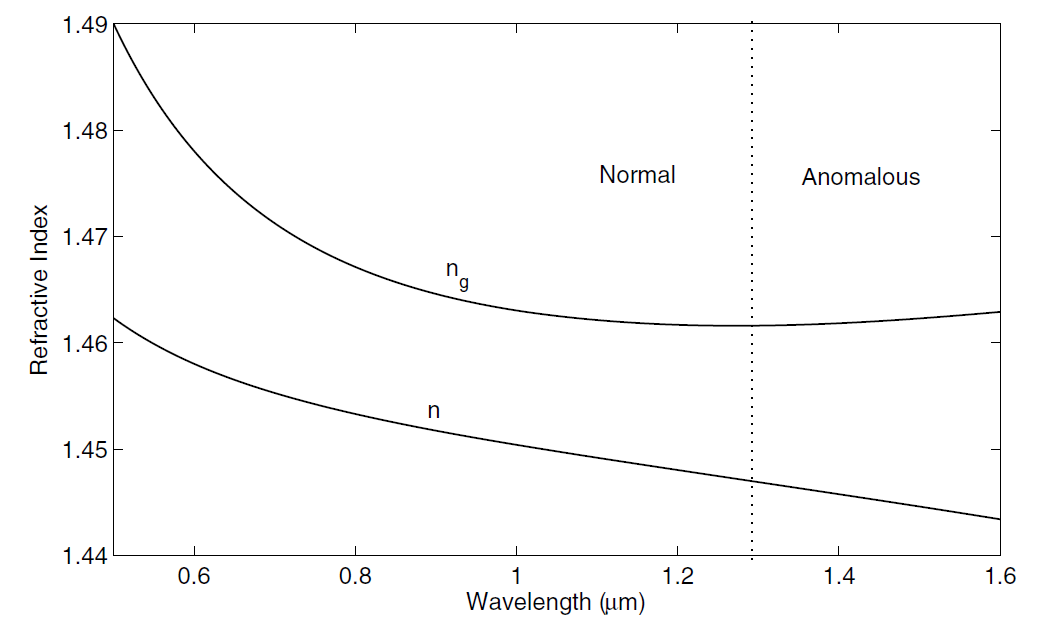
\includegraphics[width=0.6\textwidth]{images/fig1.4.PNG}
                        \caption{Variation of refractive index n and group index $n_g$ with wavelength for fused silica. $n(\omega)$ is calculated from \autoref{sellmeier equation}, $n_g(\omega)$ is calculaed from \autoref{group velocity and group index}.}
                        \label{fig1.4}
                    \end{figure}
                    
                    \begin{figure}[htbp]
                        \centering
                        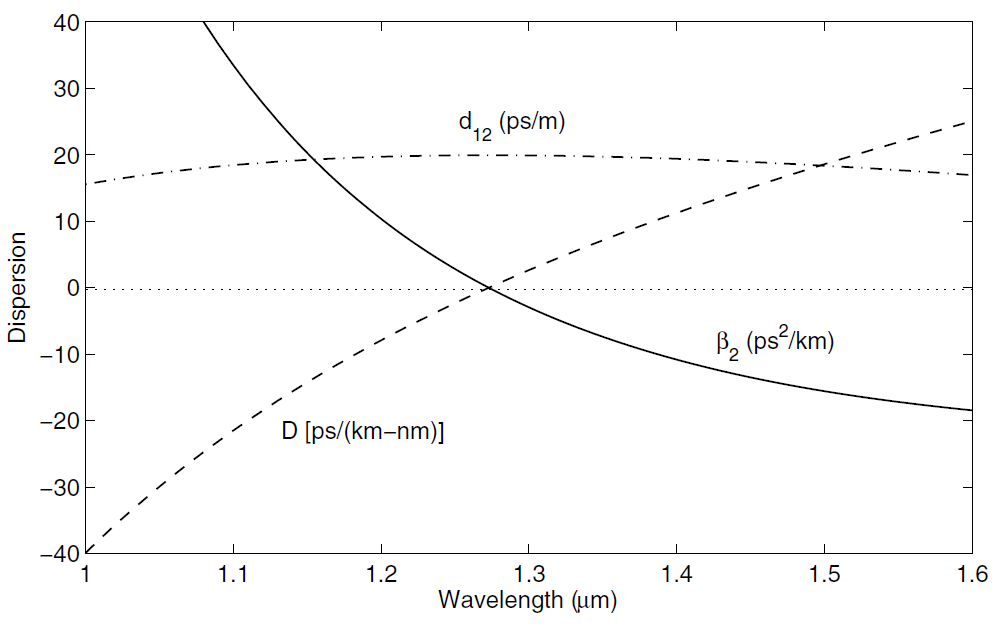
\includegraphics[width=0.6\textwidth]{images/fig1.5.PNG}
                        \caption{Variation of β2, D, and d12 with wavelength for fused silica. Both $\beta_2$ and D vanish at the zero-dispersion wavelength occurring near 1.27 $\mu m$. The $d_{12}$ here stands for $d_{12}(\lambda, 0.8\mu m)$ in \autoref{d12 definition}.}
                        \label{fig1.5}
                    \end{figure}
                    
                \item Zero dispersion wavelength $\lambda_D$, where $\beta_2$ and D are 0. Around this regime $\beta_3$ (Third Order Dispersion, TOD) in \autoref{propagation constant expansion} becomes important. 
                
                \item WHY $\lambda_D$ is different between bulked fused silica($1.27\mu m$) and actual glass fibers(typically $1.31\mu m$):
                    \SubItem{1.} Fiber core have dopants such as $GeO_2$ or $P_2O_5$.
                    \SubItem{2.} Fiber modes are confined in two directions, which discrete k number in these two directions. This geometry effect will influence dispersion.
                    \SubItem{3.} Other fiber design parameters such as core radius a and core-cladding index difference $\Delta$. Dispersion shift fibers can move $\lambda_D$ to $1.55\mu m$, where fiber loss at minium.
                    \SubItem{4.} dispersion-flattened optical fibers by multi-clad layer.
                    
                \item walk-off parameter $d_{12}$: nonlinear interaction between two optical pulses ceases
                to occur when the faster moving pulse completely walks through the slower moving pulse.
                    \begin{equation}
                        d_{12}(\lambda_1,\lambda_2) = \beta_1(\lambda_1)-\beta(\lambda_2) = v_g^{-1}(\lambda_1)-v_g^{-1}(\lambda_2)
                        \label{d12 definition}
                    \end{equation}
                    For pulses of width $T_0$, walk-off length $L_W$ defined by:
                    \begin{equation}
                        L_W = \frac{T_0}{\abs{d_{12}}}
                        \label{LW definition}
                    \end{equation}
            \end{itemize}
        
        
        \subsubsection{Polarization-Mode Dispersion}
            \begin{itemize}
                \item Even single mode fiber supports two degeneracy modes: x-polarization and y-polarization modes.
                \item cylindrical asymmetry and stress-induced anisotropy can break this degeneracy. This is called modal birefringence. 
                    \begin{equation}
                        B_m = \frac{\abs{\beta_x-\beta_y}}{k_0}=\abs{n_x-n_y}
                        \label{polarization birefringence definition}
                    \end{equation}
                \item For a given value of Bm, the two modes exchange their powers in a periodic fashion as they propagate inside the fiber with the Beat Length period
                    \begin{equation}
                        L_B = \frac{2\pi}{\abs{\beta_x-\beta_y}}=\frac{\lambda}{B_m}.
                        \label{Beat length definition}
                    \end{equation}
                    The intuition of Beat length can be illustrated by \autoref{beat lenghth illustration}.
                    \begin{figure}[htbp]
                        \centering
                        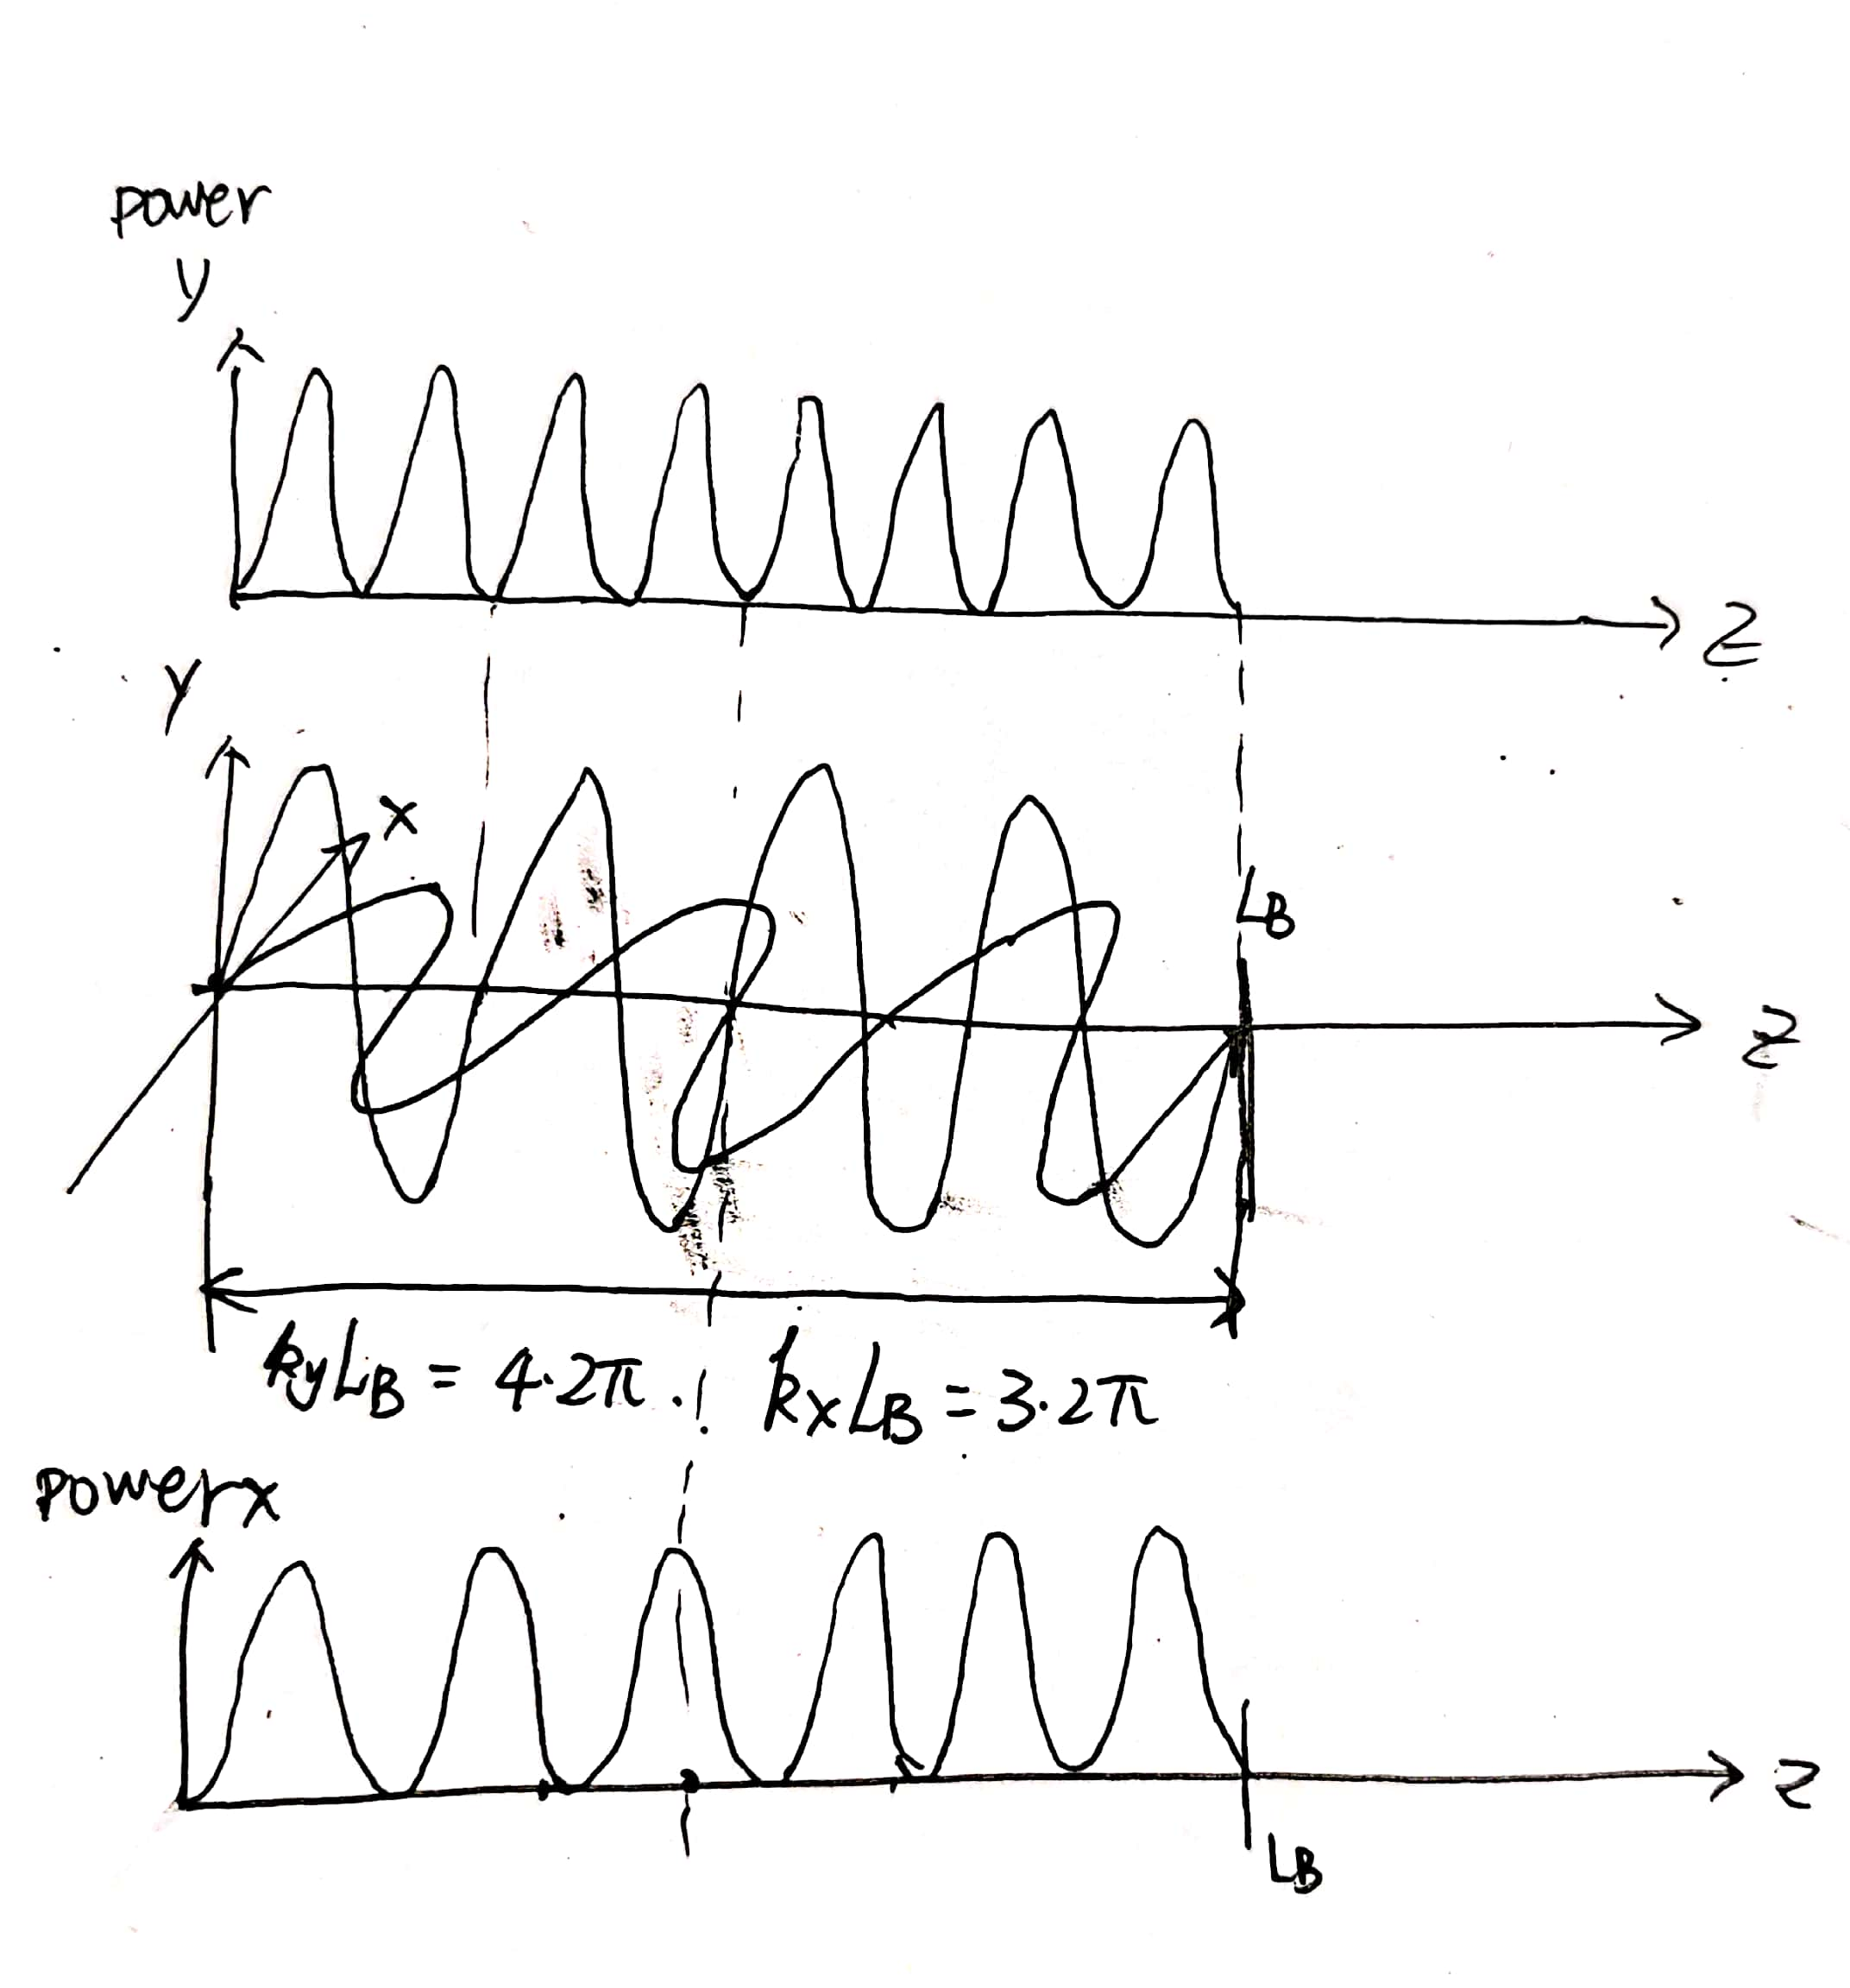
\includegraphics[width=0.6\textwidth]{images/polar_dispersion.jpg}
                        \caption{Beat length illustration}
                        \label{beat lenghth illustration}
                    \end{figure}
                    
                    \begin{figure}[htbp]
                        \centering
                        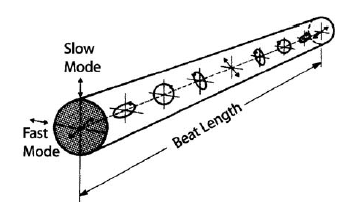
\includegraphics[width=0.6\textwidth]{images/fig1.9.PNG}
                        \caption{Evolution of state of polarization along a polarization-maintaining fiber when input signal is linearly polarized at 45 from the slow axis.}
                        \label{fig1.9}
                    \end{figure}
                    
                \item The pulse becomes broader at the output end because group velocities change $\bold{randomly}$ in response to random changes in fiber birefringence (analogous to a random-walk problem).
                    \begin{equation}
                        \Delta T = \abs{\frac{L}{v_{gx}-v_{gy}}}=L\abs{\beta_{1x}-\beta{1y}}
                    \end{equation}
                    The variance of $\Delta T$ is
                    \begin{equation}
                        \sigma_T \approx D_p \sqrt{L}.
                    \end{equation}
                    $D_p$ is PMD(Polarization-Mode Dispersion) parameter. L is travel distance.
                    
                \item polarization-maintaining fibers: induces LARGE amount of birefringence so that the FLUCTUATIONS do not significantly affect polarization.---> Which means polarization maintaining fibers can only maintain the polarization along fast or slow axis well.
            \end{itemize}
            
    \subsection{Fiber Nonlinearities}
        \begin{itemize}
            \item On a fundamental level, the origin of nonlinear response is related to aharmonic motion of bound electrons under the influence of an applied field.
            \item total polarization P induced by electric dipoles is not linear in the electric field E, but satisfies the more general relation:
                \begin{equation}
                    \frac{\boldsymbol{P}}{\epsilon_0} = \chi^{(1)} \cdot \boldsymbol{E} + \chi^{(2)} : \boldsymbol{EE} + \chi^{(3)} \vdots \boldsymbol{EEE} + \dots,
                    \label{general PE relation}
                \end{equation}
                where $\chi^{(j)}$ is jth order susceptibility. 
                \SubItem{Take special notice of the relation between \autoref{sellmeier equation} and \autoref{general PE relation}. In \autoref{sellmeier equation}, no nonlinearity is considered, only dispersion is considered. Thus \autoref{sellmeier equation} is correlated with the first term in \autoref{general PE relation}. which means:
                    \begin{equation}
                        \frac{\boldsymbol{P}}{\epsilon_0} = \chi^{(1)}(\omega) \cdot \boldsymbol{E} \iff n(\omega).
                    \end{equation}
                    The high order terms in \autoref{general PE relation} are not related with \autoref{sellmeier equation} since they are nonlinear terms. \autoref{sellmeier equation} don't show the power dependence of refractive index.
                }
                \SubItem{In general, $\chi^{(j)}$ is a (j,1)-tensor\cite{noauthor_tensor_2019} of rank j+1. The reason it is (j,1)-tensor is that this is a "mapping" coefficient taking in j-copies of 3-dim Cartesian space(i.e.$\boldsymbol{EE\dots}$) into a 1-cpoy of 3-dim Cartesian space(i.e. $\boldsymbol{P}$).}
                \SubItem{ Rank 4 tensor is a good example to illustrate the difference between convariant and contravariant indexes. Any tensor is a (p,q)-tensor with rank of p+q, where p is contravariant index, denoted as the uppper index; q is covariant index, denoted as lower index.
                    \begin{itemize}
                        \item For rank-4 tensors, typically have two types: type (3,1), such as 3rd order susceptibility $\chi^{(3)}$; and type (2,2), such as elasticity tensor\cite{noauthor_hookes_2019}.
                        \item For rank 4 type (3,1): 3rd order susceptibility $\chi^{(3)}$, has 3 contravariant index(upper index) and 1 covariant index(lower index). The mathematical formation of $\chi^{(3)}$ is
                            \begin{equation}
                                \label{illustration of chi3 as (1,3)-tensor}
                                \frac{\boldsymbol{P}^{(3)}}{\epsilon_0} = \chi^{(3)} \vdots \boldsymbol{EEE}.
                            \end{equation}
                        Expand $\boldsymbol{P}^{(3)}$ in x,y,z directions (Using Einstein summation notation, sum over same notations, which are $ ijk \in \{x,y,z\} $ here):
                            \begin{equation}
                                \begin{cases}
                                P^{(3)}_x /\epsilon_0 = {\chi^{(3)}}_x^{ijk}E_i E_j E_k\\
                                P^{(3)}_y / \epsilon_0 = {\chi^{(3)}}_y^{ijk}E_i E_j E_k\\
                                P^{(3)}_z /\epsilon_0 = {\chi^{(3)}}_z^{ijk}E_i E_j E_k.
                                \end{cases}
                            \end{equation}
                        Thus $\chi^{(3)}$ is type (3,1) rank 4-tensor with 3 contravariant indexes and 1 covariant index.
                        \item For rank 4 type (2,2): elasticity tensor $\boldsymbol{c}$ \cite{noauthor_hookes_2019}, relates strain tensor $\boldsymbol{\epsilon}$ (in lieu of the displacement X in F=-kX) and the stress tensor $\boldsymbol{\sigma}$ (replacing the restoring force F) as
                            \begin{equation}
                                \boldsymbol{\sigma} = - \boldsymbol{c} \boldsymbol{\epsilon},
                                \label{Hooke's law in tensor form}
                            \end{equation}
                            where strain tensor $\boldsymbol{\epsilon}$ and stress tensor $\boldsymbol{\sigma}$ are order 2 tensor with 3-dim.
                                \begin{multicols}{2}
                                \setlength{\columnseprule}{0pt}
                                \noindent
                                    \begin{equation}
                                        \boldsymbol{\epsilon} = 
                                            \begin{pmatrix}
                                                \epsilon_{xx} & \epsilon_{xy} & \epsilon_{xz}\\
                                                \epsilon_{yx} & \epsilon_{yy} & \epsilon_{yz}\\
                                                \epsilon_{zx} & \epsilon_{zy} & \epsilon_{zz}
                                            \end{pmatrix}
                                    \end{equation}
                                    \begin{equation}
                                        \boldsymbol{\sigma} = 
                                            \begin{pmatrix}
                                                \sigma_{xx} & \sigma_{xy} & \sigma_{xz}\\
                                                \sigma_{yx} & \sigma_{yy} & \sigma_{yz}\\
                                                \sigma_{zx} & \sigma_{zy} & \sigma_{zz}
                                            \end{pmatrix}.
                                    \end{equation}
                                \end{multicols}
                            The relation between $\boldsymbol{\epsilon}$ and $\boldsymbol{\sigma}$ is connected by $\boldsymbol{c}$ in the form of
                                \begin{equation}
                                    \sigma_{ij} = {c_{ij}}^{kl}\epsilon_{kl},
                                \end{equation}
                            where common indexes to sum up are $ kl \in \{x,y,z\} $ this time. \\
                            Thus $\boldsymbol{c}$ is type (2,2) rank 4-tensor with 2 contravariant indexes and 2 covariant indexes.
                    \end{itemize}
                }
            \item second-order susceptibility: second-harmonic generation; sum-frequency generation. nonzero only for media that lack an inversion symmetry at the molecular level. 
                \SubItem{Silica doesn't have this in-symmetry. Only electric-quadrupole and magnetic-dipole moments can generate weak second-order nonlinear effects.Defects or color centers inside the fiber core can also contribute to second-harmonic generation.}
            \item third-order susceptibility: third-harmonic generation; four-wave mixing; nonlinear refraction.
                \SubItem{Unless special efforts are made to achieve \textbf{phase matching}, the nonlinear processes that involve generation of new frequencies (e.g., third-harmonic generation and four-wave mixing) are not efficient in optical fibers.\label{Why nonlinear refraction most important} }
        \end{itemize}
        
        \subsubsection{Nonlinear Refraction}
            \begin{itemize}
                \item As \ref{Why nonlinear refraction most important} said, silica fiber doesn't have second order nonlinearity, thus refractive index in the simplest form is:
                    \begin{equation}
                        \Tilde{n}(\omega,I) = n(\omega) + n_2 I = n + \overline{n}_2\abs{\boldsymbol{E}}^2,
                        \label{simplest nonlinear refractive index form}
                    \end{equation}
                    which is isotropic(This is very important!). In \autoref{simplest nonlinear refractive index form}, $n(\omega)$ is the linear part (This linear doesn't mean Taylor expansion to 1st order, this linear means a linear process, which refractive index has no relation with electric field) given by \autoref{sellmeier equation}. $\overline{n}_2$ is the average $n_2$ over fiber cross-section. Notice $\abs{\boldsymbol{E}}^2$ also evolves some kind of average over the fiber cross-section.
                    
                \item $\overline{n}_2$ is nonlinear index coefficient, related to  $\chi^{(3)}$ by (will be derived later)
                    \begin{equation}
                        \overline{n}_2 = \frac{3}{8n} \Re({ \chi^{(3)} }_x^{xxx}).
                        \label{n2 bar relation with chi3}
                    \end{equation}
                    Notice that optical field E is assumed to be linearly polarized so that only one component ${ \chi^{(3)} }_x^{xxx}$ contributes. Other components can affect polarization by nonlinear birefringence.
                \item Self-phase modulation (SPM):
            \end{itemize}


% \subsubsection{effective red and blue detune}


% \section{Coupling mode equation}


% \section{Soliton generation}
% \subsection{modulation instability}


% \subsection{Turing pattern}
% \subsection{Bright cavity soliton}
% \subsection{Bright soliton molecules}
% \subsection{Breathing solitons}


% \section{Induction Proofs}
% \subsection{Ordinary Induction}
% \begin{exercise} Prove, for all natural numbers $n$, that 
% \begin{equation} \sum_{k=0}^n k = 1 + 2 + 3 + \cdots + n = \dfrac{n(n+1)}{2}
% \label{eq:Pn}\end{equation}
% \end{exercise}

% \begin{proof}
% We prove this by induction on $n\in\N$.  In the base case, $n=0$, and \eqref{eq:Pn} becomes
% $$\sum_{k=0}^n k = \sum_{k=0}^0 k = 0 = \dfrac{0(1)}{2} = \dfrac{n(n+1)}{2}$$

% Now, let $n>0$ be arbitrary, and assume \eqref{eq:Pn}.
% We show $\displaystyle \sum_{k=0}^{n+1} k = \dfrac{(n+1)(n+2)}{2}$.
% To that end note 
% \begin{align*}
% 	\sum_{k=0}^{n+1} k &= \left(\sum_{k=0}^{n} k\right) + (n+1) &\mbox{(sum definition)}\\
% 	&= \frac{n(n+1)}{2} + (n+1) &\mbox{(induction hypothesis)}
% 	\\
% 	&= \frac{n(n+1)}{2} + \frac{2n+2}{2} &\mbox{(common denominator)}
% 	\\
% 	&= \frac{n^2 +n}{2} + \frac{2n+2}{2} &\mbox{(distribute)}
% 	\\
% 	&= \frac{n^2 +3n + 2}{2} &\mbox{(combine like terms)}
% 	\\
% 	&= \frac{(n+1)(n+2)}{2} & \mbox{(factor the numerator)}\\
% \end{align*}

% In all cases, \eqref{eq:Pn} is true, so $\forall n\in \N$, 
% $\Disp \sum_{k=0}^n k = \dfrac{n(n+1)}{2}$
% \end{proof}
\bibliographystyle{IEEEtran}
\bibliography{references.bib}
\end{document}
